\documentclass[11pt, a4paper]{article}
\usepackage[left=2.5cm, right=2.5cm, top=3cm, bottom=3cm]{geometry}
\usepackage{tikz}
\usetikzlibrary{arrows.meta, positioning, shapes.geometric, shapes.symbols,
                fit, backgrounds, shadows.blur, calc}
\usepackage{xcolor}
\usepackage{fancyhdr}
\usepackage{booktabs}
\usepackage{longtable}
\usepackage{array}
\usepackage{enumitem}
\usepackage{listings}
\usepackage{tcolorbox}
\tcbuselibrary{skins, breakable}
\usepackage[hidelinks]{hyperref}
\usepackage{graphicx}
\usepackage{amssymb}
\usepackage{microtype}
\setlength{\emergencystretch}{3em}

% ── Colours ────────────────────────────────────────────────────────────────────
\definecolor{mea-blue}{RGB}{0,82,155}
\definecolor{mea-light}{RGB}{220,235,255}
\definecolor{vsecc-green}{RGB}{0,140,60}
\definecolor{vsecc-light}{RGB}{210,245,220}
\definecolor{ev-orange}{RGB}{210,95,0}
\definecolor{ev-light}{RGB}{255,235,200}
\definecolor{pc-gray}{RGB}{70,70,90}
\definecolor{pc-light}{RGB}{230,230,240}
\definecolor{internet-color}{RGB}{150,150,200}
\definecolor{code-bg}{RGB}{245,245,250}
\definecolor{warn-bg}{RGB}{255,248,220}
\definecolor{warn-border}{RGB}{210,160,0}
\definecolor{pass-bg}{RGB}{240,255,240}
\definecolor{fail-bg}{RGB}{255,240,240}
\definecolor{passgreen}{RGB}{34,139,34}
\definecolor{failred}{RGB}{200,0,0}
\definecolor{warnorange}{RGB}{200,100,0}
\definecolor{skipgray}{RGB}{120,120,120}

% ── Header / footer ────────────────────────────────────────────────────────────
\pagestyle{fancy}
\fancyhf{}
\lhead{\textcolor{mea-blue}{\textbf{MEA OCPP 1.6}} — vSECC Test Manual}
\rhead{\thepage}
\renewcommand{\headrulewidth}{0.6pt}

% ── Listings (code blocks) ─────────────────────────────────────────────────────
\lstset{
  basicstyle=\small\ttfamily,
  backgroundcolor=\color{code-bg},
  frame=single,
  framesep=4pt,
  rulecolor=\color{gray!40},
  breaklines=true,
  breakatwhitespace=true,
  postbreak=\mbox{\textcolor{gray}{$\hookrightarrow$}\space},
  tabsize=2,
  showstringspaces=false,
  columns=fullflexible,
}

% ── tcolorbox styles ───────────────────────────────────────────────────────────
\tcbset{
  noteboxstyle/.style={
    enhanced, breakable,
    colback=warn-bg, colframe=warn-border,
    fonttitle=\bfseries\small, title=#1,
    left=4pt, right=4pt, top=4pt, bottom=4pt,
  },
  tipboxstyle/.style={
    enhanced, breakable,
    colback=pass-bg, colframe=passgreen!60,
    fonttitle=\bfseries\small, title=#1,
    left=4pt, right=4pt, top=4pt, bottom=4pt,
  },
}

\newcolumntype{L}[1]{>{\raggedright\arraybackslash}p{#1}}
\newcolumntype{C}[1]{>{\centering\arraybackslash}p{#1}}

% ────────────────────────────────────────────────────────────────────────────────
\begin{document}

\begin{titlepage}
  \centering
  \vspace*{2cm}
  {\color{mea-blue}\rule{\linewidth}{2pt}}\\[0.6em]
  {\Huge\bfseries MEA OCPP 1.6 Compliance Test}\\[0.4em]
  {\LARGE Setup \& Run Manual}\\[0.4em]
  {\color{mea-blue}\rule{\linewidth}{2pt}}\\[2em]
  {\large Vector vSECC.single Board vs MEA CSMS Sandbox}\\[0.5em]
  {\large Sections 2--11 $\mid$ Direct connection (no proxy)}\\[3em]
  \begin{tabular}{ll}
    \textbf{Device under test} & Vector vSECC.single Board \\
    \textbf{Device IP}         & 192.168.1.166 \\
    \textbf{OCPP version}      & 1.6 (JSON over WebSocket) \\
    \textbf{CP identity}       & \texttt{rddQC4000001} \\
    \textbf{CSMS}              & \texttt{wss://ocpp.measandbox.com:2930} \\
    \textbf{Test PC}           & 192.168.111.185 (+ alias 192.168.1.200/24) \\
    \textbf{Document}          & \texttt{docs/vsecc\_test\_manual.pdf} \\
  \end{tabular}
  \vfill
  {\small MEA-V2G Project --- Automated Test Infrastructure}
\end{titlepage}

\tableofcontents
\newpage

% ════════════════════════════════════════════════════════════════════════════════
\section{System Overview}
% ════════════════════════════════════════════════════════════════════════════════

\subsection{Architecture Diagram}

\begin{figure}[h]
\centering
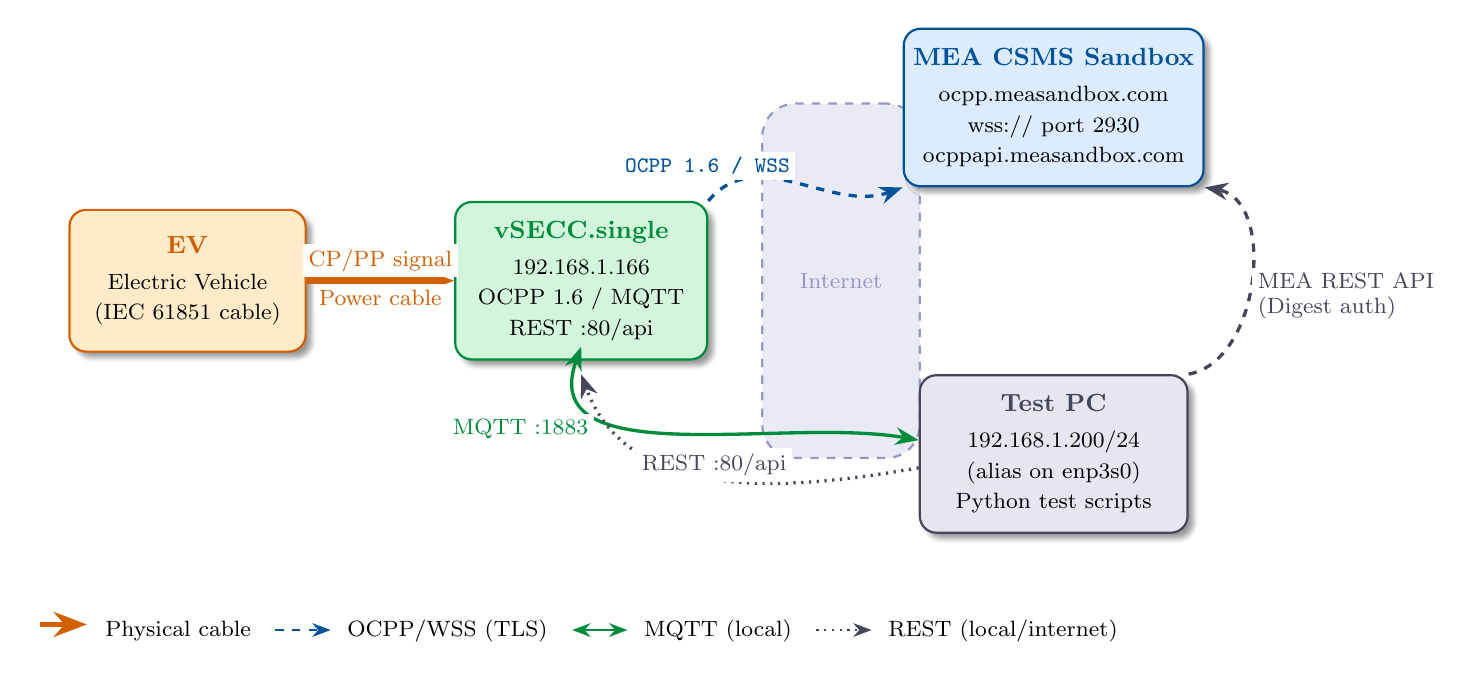
\begin{tikzpicture}[
  >=Stealth,
  node distance = 0pt,
  every node/.style = {font=\small},
  % Box styles
  evbox/.style    = {draw=ev-orange,    fill=ev-light,    thick, rounded corners=6pt,
                     minimum width=3cm,   minimum height=1.8cm, align=center,
                     blur shadow={shadow blur steps=5}},
  vseccbox/.style = {draw=vsecc-green,  fill=vsecc-light, thick, rounded corners=6pt,
                     minimum width=3.2cm, minimum height=2cm,   align=center,
                     blur shadow={shadow blur steps=5}},
  pcbox/.style    = {draw=pc-gray,      fill=pc-light,    thick, rounded corners=6pt,
                     minimum width=3.4cm, minimum height=2cm,   align=center,
                     blur shadow={shadow blur steps=5}},
  csmsbox/.style  = {draw=mea-blue,     fill=mea-light,   thick, rounded corners=6pt,
                     minimum width=3.4cm, minimum height=2cm,   align=center,
                     blur shadow={shadow blur steps=5}},
  cloudbox/.style = {draw=internet-color, fill=internet-color!20, thick, dashed,
                     rounded corners=12pt, minimum width=4cm, minimum height=1cm,
                     align=center},
  % Arrow styles
  cabarrow/.style = {->, ultra thick, ev-orange},
  ocpparrow/.style= {->, thick, mea-blue, dashed},
  mqttarrow/.style= {<->, thick, vsecc-green},
  restbarrow/.style= {->, thick, pc-gray, dotted},
  labelstyle/.style = {font=\footnotesize, fill=white, inner sep=2pt},
]

% ── Nodes ──────────────────────────────────────────────────────────────────────

% EV (left)
\node[evbox] (ev) at (0, 0) {
  \textcolor{ev-orange}{\textbf{EV}}\\[2pt]
  \footnotesize Electric Vehicle\\
  \footnotesize (IEC 61851 cable)
};

% vSECC (centre)
\node[vseccbox] (vsecc) at (5, 0) {
  \textcolor{vsecc-green}{\textbf{vSECC.single}}\\[2pt]
  \footnotesize 192.168.1.166\\
  \footnotesize OCPP 1.6 / MQTT\\
  \footnotesize REST :80/api
};

% MEA CSMS (top right)
\node[csmsbox] (csms) at (11, 2.2) {
  \textcolor{mea-blue}{\textbf{MEA CSMS Sandbox}}\\[2pt]
  \footnotesize ocpp.measandbox.com\\
  \footnotesize wss:// port 2930\\
  \footnotesize ocppapi.measandbox.com
};

% Test PC (bottom right)
\node[pcbox] (pc) at (11, -2.2) {
  \textcolor{pc-gray}{\textbf{Test PC}}\\[2pt]
  \footnotesize 192.168.1.200/24\\
  \footnotesize (alias on enp3s0)\\
  \footnotesize Python test scripts
};

% Internet cloud (background behind CSMS and arrows going right)
\begin{scope}[on background layer]
  \node[cloudbox, minimum width=2cm, minimum height=4.5cm]
    at (8.3, 0) {\textcolor{internet-color}{\footnotesize Internet}};
\end{scope}

% ── Arrows ─────────────────────────────────────────────────────────────────────

% EV → vSECC  (physical cable)
\draw[cabarrow, line width=2.5pt]
  (ev.east) -- (vsecc.west)
  node[labelstyle, midway, above] {CP/PP signal}
  node[labelstyle, midway, below] {Power cable};

% vSECC → CSMS  (OCPP/TLS)
\draw[ocpparrow, line width=1.2pt]
  (vsecc.north east) to[out=50, in=200]
  node[labelstyle, midway, above left] {\texttt{OCPP 1.6 / WSS}}
  (csms.south west);

% PC → CSMS  (MEA REST API)
\draw[ocpparrow, line width=1.2pt, pc-gray]
  (pc.north east) to[out=10, in=350]
  node[labelstyle, midway, right] {\footnotesize MEA REST API}
  node[labelstyle, midway, right, yshift=-10pt] {\footnotesize (Digest auth)}
  (csms.south east);

% vSECC ↔ PC  (MQTT + REST local)
\draw[mqttarrow, line width=1.2pt]
  ([yshift=5pt]vsecc.south) to[out=250, in=170]
  node[labelstyle, near start, below left] {\footnotesize MQTT :1883}
  ([yshift=5pt]pc.west);

\draw[restbarrow, line width=1.2pt]
  ([yshift=-5pt]pc.west) to[out=190, in=290]
  node[labelstyle, near end, below right] {\footnotesize REST :80/api}
  ([yshift=-5pt]vsecc.south);

% ── Legend ─────────────────────────────────────────────────────────────────────
\node[align=left, font=\footnotesize] at (5, -4.4) {
  \tikz\draw[cabarrow, line width=2pt] (0,0)--(0.6,0); \ Physical cable\quad
  \tikz\draw[ocpparrow] (0,0)--(0.7,0); \ OCPP/WSS (TLS)\quad
  \tikz\draw[mqttarrow] (0,0)--(0.7,0); \ MQTT (local)\quad
  \tikz\draw[restbarrow] (0,0)--(0.7,0); \ REST (local/internet)
};

\end{tikzpicture}
\caption{MEA vSECC Test System --- Network and Protocol Topology}
\label{fig:topology}
\end{figure}

\subsection{How it works}

The vSECC.single Board handles CP signalling, SLAC, and ISO~15118
autonomously. It connects directly to the MEA CSMS sandbox over a TLS
WebSocket (\texttt{OCPP~1.6~JSON}). The test PC sits on the same local
subnet and:
\begin{itemize}[nosep]
  \item Observes OCPP events via the \textbf{vSECC MQTT broker} on port 1883.
  \item Reads vSECC state via the \textbf{vSECC REST API} on port 80.
  \item Sends OCPP commands (RemoteStart, Reset, ReserveNow, \ldots) via the
        \textbf{MEA REST API} over HTTPS.
\end{itemize}

No OCPP proxy is used. All OCPP traffic runs directly between vSECC and CSMS.

% ════════════════════════════════════════════════════════════════════════════════
\section{Hardware Requirements}
% ════════════════════════════════════════════════════════════════════════════════

\begin{tabular}{L{4cm} L{10cm}}
\toprule
\textbf{Component} & \textbf{Details} \\
\midrule
Vector vSECC.single & Firmware with OCPP~1.6 JSON; MQTT broker enabled \\
Test PC             & Linux, Python~3.11+, \texttt{pdflatex} \\
Network switch      & Connects vSECC and PC on the \texttt{192.168.1.x} subnet \\
EV (optional)       & Required only for EV-plug test items; all API tests run without it \\
\bottomrule
\end{tabular}

\bigskip
The vSECC must be pre-configured with:
\begin{itemize}[nosep]
  \item OCPP endpoint: \texttt{wss://ocpp.measandbox.com:2930/EV/Srv/JSON/1.6/rddQC4000001}
  \item CP identity: \texttt{rddQC4000001}
  \item MQTT broker: built-in at \texttt{192.168.1.166:1883}
\end{itemize}

% ════════════════════════════════════════════════════════════════════════════════
\section{Network Setup}
% ════════════════════════════════════════════════════════════════════════════════

\subsection{Physical wiring}

Connect \texttt{enp3s0} on the Test PC to the same switch as the vSECC ETH
port. The PC gets a DHCP address on \texttt{192.168.111.0/24}.
Because the vSECC is on \texttt{192.168.1.x}, add an alias:

\begin{lstlisting}[language=bash]
sudo ip addr add 192.168.1.200/24 dev enp3s0
\end{lstlisting}

\begin{tcolorbox}[noteboxstyle={Note}]
This alias is \textbf{not persistent} across reboots or network restarts.
Re-run the command each session, or make it persistent (see below).
\end{tcolorbox}

\subsection{Verify connectivity}

\begin{lstlisting}[language=bash]
ping -c 3 192.168.1.166                   # vSECC should reply
curl -s http://192.168.1.166/api | head   # should return JSON (not timeout)
\end{lstlisting}

\subsection{Make the alias persistent}

Create \texttt{/etc/networkd-dispatcher/routable.d/10-vsecc-alias}:

\begin{lstlisting}[language=bash]
#!/bin/bash
ip addr add 192.168.1.200/24 dev enp3s0 2>/dev/null || true
\end{lstlisting}

\begin{lstlisting}[language=bash]
sudo chmod +x /etc/networkd-dispatcher/routable.d/10-vsecc-alias
\end{lstlisting}

% ════════════════════════════════════════════════════════════════════════════════
\section{Software Prerequisites}
% ════════════════════════════════════════════════════════════════════════════════

\subsection{Python packages}

\begin{lstlisting}[language=bash]
.venv/bin/pip install requests paho-mqtt
\end{lstlisting}

\subsection{pdflatex (for PDF reports)}

\begin{lstlisting}[language=bash]
sudo apt install texlive-latex-base texlive-latex-extra \
                 texlive-fonts-recommended
pdflatex --version   # verify
\end{lstlisting}

\subsection{MQTT monitor (optional, for debugging)}

\begin{lstlisting}[language=bash]
sudo apt install mosquitto-clients

# Subscribe to all relevant vSECC topics:
mosquitto_sub -h 192.168.1.166 -p 1883 -u vector -P vector \
  -t "vsecc/connector/#" \
  -t "vsecc/ocpp_connection_status" -v
\end{lstlisting}

% ════════════════════════════════════════════════════════════════════════════════
\section{Configuration}
% ════════════════════════════════════════════════════════════════════════════════

All parameters are constants at the top of each test file.

\begin{center}
\begin{tabular}{L{4.5cm} L{3.5cm} L{6cm}}
\toprule
\textbf{Constant} & \textbf{Default} & \textbf{Description} \\
\midrule
\texttt{VSECC\_BASE}        & \texttt{http://192.168.1.166/api} & vSECC REST endpoint \\
\texttt{MQTT\_HOST}         & \texttt{192.168.1.166}            & vSECC MQTT broker host \\
\texttt{CP\_ID}             & \texttt{rddQC4000001}             & Charge point identity \\
\texttt{RFID\_TAG}          & \texttt{RFID\_TEST}               & RFID tag used for auth \\
\texttt{EV\_WAIT\_SEC}      & \texttt{60}                       & Seconds to wait for EV plug event \\
\texttt{BOOT\_WAIT\_SEC}    & \texttt{90}                       & Seconds to wait after Hard Reset \\
\texttt{LOCAL\_STOP\_WAIT\_SEC} & \texttt{30}                   & Seconds to wait for RFID tap to stop session \\
\texttt{EXPIRY\_WAIT\_SEC}  & \texttt{90}                       & Seconds to wait for reservation expiry (sec.~5) \\
\bottomrule
\end{tabular}
\end{center}

\bigskip
\textbf{Without a real EV} --- set \texttt{EV\_WAIT\_SEC~=~0}.
EV-dependent items record \textbf{WARN} immediately instead of blocking.

\begin{lstlisting}[language=bash]
sed -i 's/^EV_WAIT_SEC = 60/EV_WAIT_SEC = 0/' \
  tests/vsecc/test_mea_sectionN.py
\end{lstlisting}

% ════════════════════════════════════════════════════════════════════════════════
\section{Running the Tests}
% ════════════════════════════════════════════════════════════════════════════════

All test scripts are standalone Python programs (not pytest).
Run from the \textbf{project root}:

\begin{lstlisting}[language=bash]
.venv/bin/python3 tests/vsecc/test_mea_sectionN.py
\end{lstlisting}

Results are saved automatically to \texttt{tex/vsecc\_sectionN\_results.json}.

\subsection{Section guide}

\begin{center}
\renewcommand{\arraystretch}{1.3}
\begin{tabular}{C{1cm} L{4cm} C{2.2cm} L{7cm}}
\toprule
\textbf{Sec.} & \textbf{Title} & \textbf{EV needed} & \textbf{Notes} \\
\midrule
1  & Charger Configuration & No            & GetConfiguration, ChangeConfiguration, identity checks \\
2  & Auto Charge           & \textbf{Yes}  & All 21 items require EV plug for auto-charge flow \\
3  & Normal Operation      & \textbf{Yes}  & Local RFID + RemoteStart; 16 of 19 items need EV \\
4  & Reset Check           & \textbf{Yes}  & 15 of 21 items need EV (charging during reset) \\
5  & Reservation           & \textbf{Yes}  & Flow 3 (9 items) needs EV; Flows 1--2 work without \\
6  & Charging Profile      & \textbf{Yes}  & All charging-profile items need active EV session \\
7  & Abnormal Operation    & \textbf{Yes}  & E-stop, door, power loss all require EV plugged in \\
8  & Dual Connector        & N/A           & All SKIP — single connector device \\
9  & V2G / BPT             & Partial       & Config items (9.1--9.3) no EV; BPT items (9.4) need EV \\
10 & CSMS Commands         & No            & All 23 commands testable via REST without EV \\
11 & Performance           & No            & Reconnect time only; 3$\times$ Hard Reset \\
\bottomrule
\end{tabular}
\end{center}

\begin{tcolorbox}[noteboxstyle={Important: Run with EV for meaningful compliance results}]
Sections 2--7 have the majority of their items dependent on a physical EV
being connected. Without EV, these items record \textbf{WARN} and
cannot demonstrate compliance. Connect a real EV before running
sections 2--7 to obtain \textbf{PASS} results for the full test suite.
\end{tcolorbox}

\subsection{Run without EV (API connectivity check only)}

Sections 2--7 will produce mostly \textbf{WARN} results without an EV.
Use this mode only to verify that the vSECC is reachable and the MEA API
is responding correctly before a full EV session.

\begin{lstlisting}[language=bash]
for s in 1 2 3 4 5 6 7 8 9 10 11; do
  sed -i 's/^EV_WAIT_SEC = 60/EV_WAIT_SEC = 0/' \
    tests/vsecc/test_mea_section${s}.py 2>/dev/null
  echo "=== Section $s ==="
  .venv/bin/python3 tests/vsecc/test_mea_section${s}.py
done
\end{lstlisting}

\subsection{Run with real EV (recommended for compliance)}

This is the recommended mode for a proper compliance test run.
Connect an EV to the vSECC connector before starting.

\begin{lstlisting}[language=bash]
# Restore EV wait timeout (60 s per plug event):
for s in 2 3 4 5 6 7; do
  sed -i 's/^EV_WAIT_SEC = 0/EV_WAIT_SEC = 60/' \
    tests/vsecc/test_mea_section${s}.py 2>/dev/null
done

# Run all sections:
for s in 1 2 3 4 5 6 7 8 9 10 11; do
  echo "=== Section $s ==="
  .venv/bin/python3 tests/vsecc/test_mea_section${s}.py
done
\end{lstlisting}

% ════════════════════════════════════════════════════════════════════════════════
\section{Running With a Real EV --- Step by Step}
% ════════════════════════════════════════════════════════════════════════════════

\subsection{Pre-run checklist}

\begin{itemize}[nosep]
  \item[$\square$] vSECC powered on; OCPP LED green (connected to MEA CSMS).
  \item[$\square$] Network alias active:
        \texttt{ip addr show enp3s0 | grep 192.168.1.200}
  \item[$\square$] EV not at 100\% SoC (must be willing to accept a session).
  \item[$\square$] RFID card \texttt{RFID\_TEST} registered in MEA CSMS,
        or use a physical authorised card and update \texttt{RFID\_TAG}.
  \item[$\square$] \texttt{EV\_WAIT\_SEC = 60} in the test file.
\end{itemize}

\subsection{Section 3 — Normal Operation}

\begin{center}
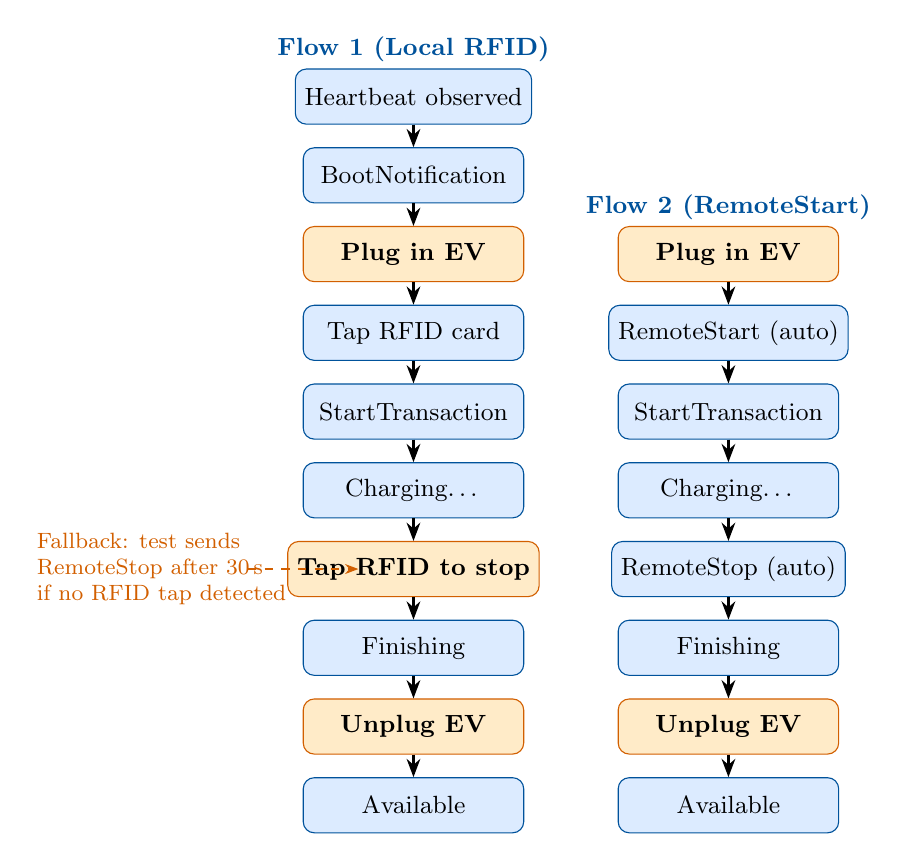
\begin{tikzpicture}[
  >=Stealth,
  box/.style={draw, rounded corners=4pt, minimum width=2.8cm,
              minimum height=0.7cm, align=center, font=\small},
  action/.style={box, fill=ev-light, draw=ev-orange},
  auto/.style={box, fill=mea-light, draw=mea-blue},
  arrow/.style={->, thick},
]
\node[auto]   (h)  at (0,0)    {Heartbeat observed};
\node[auto]   (b)  at (0,-1)   {BootNotification};
\node[action] (p1) at (0,-2)   {\textbf{Plug in EV}};
\node[auto]   (rf) at (0,-3)   {Tap RFID card};
\node[auto]   (st) at (0,-4)   {StartTransaction};
\node[auto]   (ch) at (0,-5)   {Charging\ldots};
\node[action] (s1) at (0,-6)   {\textbf{Tap RFID to stop}};
\node[auto]   (fi) at (0,-7)   {Finishing};
\node[action] (u1) at (0,-8)   {\textbf{Unplug EV}};
\node[auto]   (av) at (0,-9)   {Available};
\node[action] (p2) at (4,-2)   {\textbf{Plug in EV}};
\node[auto]   (rs) at (4,-3)   {RemoteStart (auto)};
\node[auto]   (st2)at (4,-4)   {StartTransaction};
\node[auto]   (ch2)at (4,-5)   {Charging\ldots};
\node[auto]   (rs2)at (4,-6)   {RemoteStop (auto)};
\node[auto]   (fi2)at (4,-7)   {Finishing};
\node[action] (u2) at (4,-8)   {\textbf{Unplug EV}};
\node[auto]   (av2)at (4,-9)   {Available};

\foreach \a/\b in {h/b, b/p1, p1/rf, rf/st, st/ch, ch/s1, s1/fi, fi/u1, u1/av}
  \draw[arrow] (\a) -- (\b);
\foreach \a/\b in {p2/rs, rs/st2, st2/ch2, ch2/rs2, rs2/fi2, fi2/u2, u2/av2}
  \draw[arrow] (\a) -- (\b);

\node[font=\small\bfseries] at (0,-0.4) {};
\node[font=\small\bfseries, mea-blue] at (0, 0.6)  {Flow 1 (Local RFID)};
\node[font=\small\bfseries, mea-blue] at (4, -1.4) {Flow 2 (RemoteStart)};

\node[font=\footnotesize, align=left, ev-orange] at (-3.2, -6)
  {Fallback: test sends\\RemoteStop after 30\,s\\if no RFID tap detected};
\draw[->, dashed, ev-orange] (-2.1, -6) -- (-0.7, -6);
\end{tikzpicture}
\end{center}

\subsection{Section 4 --- Reset Check}

After items \textbf{4.1} and \textbf{4.18} (Hard Reset), the vSECC physically
reboots. The test waits up to \texttt{BOOT\_WAIT\_SEC} (default 90\,s) for
the OCPP LED to go green before continuing. No manual action is required;
simply wait.

\subsection{Section 7 --- Abnormal Operation}

Some items require physical interaction with the vSECC hardware:

\begin{center}
\begin{tabular}{C{1.5cm} L{4cm} L{8cm}}
\toprule
\textbf{Item} & \textbf{Action} & \textbf{Detail} \\
\midrule
7.4 & Press E-stop    & Press the emergency stop button on the vSECC enclosure \\
7.5 & Open door       & Open the vSECC enclosure door (if door sensor fitted) \\
7.6 & Power loss      & Simulated via Hard Reset (automatic) \\
7.7 & Local list      & Automatic via SendLocalList REST call \\
\bottomrule
\end{tabular}
\end{center}

If a hardware action cannot be performed, the item records \textbf{WARN}.

% ════════════════════════════════════════════════════════════════════════════════
\section{Building PDF Reports}
% ════════════════════════════════════════════════════════════════════════════════

After running a test (which saves \texttt{tex/vsecc\_sectionN\_results.json}):

\begin{lstlisting}[language=bash]
# Single section:
.venv/bin/python3 tests/vsecc/generate_section5_report.py

# All sections at once:
for s in 1 2 3 4 5 6 7 8 9 10 11; do
  .venv/bin/python3 tests/vsecc/generate_section${s}_report.py
done
\end{lstlisting}

Output files are written to the \texttt{tex/} directory:

\begin{center}
\begin{tabular}{ll}
\toprule
\textbf{File} & \textbf{Section} \\
\midrule
\texttt{tex/vsecc\_section1\_report.pdf}  & Section 1: Charger Configuration \\
\texttt{tex/vsecc\_section2\_report.pdf}  & Section 2: Auto Charge \\
\texttt{tex/vsecc\_section3\_report.pdf}  & Section 3: Normal Operation \\
$\vdots$ & $\vdots$ \\
\texttt{tex/vsecc\_section11\_report.pdf} & Section 11: Performance \\
\bottomrule
\end{tabular}
\end{center}

% ════════════════════════════════════════════════════════════════════════════════
\section{Interpreting Results}
% ════════════════════════════════════════════════════════════════════════════════

\subsection{Result codes}

\begin{center}
\begin{tabular}{C{2cm} L{11cm}}
\toprule
\textbf{Status} & \textbf{Meaning} \\
\midrule
\textcolor{passgreen}{\textbf{PASS}} &
  Command accepted / MQTT event observed as expected. \\
\textcolor{failred}{\textbf{FAIL}} &
  Command rejected, or REST endpoint returned an HTTP error. \\
\textcolor{warnorange}{\textbf{WARN}} &
  Event not observed within the timeout, or a physical step was required
  but not performed (no EV connected, no RFID tap, etc.). \\
\textcolor{skipgray}{\textbf{SKIP}} &
  Test not applicable (Section~8: dual-connector tests on a
  single-connector device). \\
\bottomrule
\end{tabular}
\end{center}

\subsection{Known MEA sandbox limitations}

The following REST endpoints return HTTP~404 on the MEA sandbox.
These FAILs reflect API coverage, \textbf{not} vSECC compliance issues.

\begin{center}
\begin{tabular}{L{4.5cm} L{7cm} C{2cm}}
\toprule
\textbf{OCPP message} & \textbf{MEA REST endpoint} & \textbf{Status} \\
\midrule
TriggerMessage       & \texttt{/remote/triggerMessage}         & \textcolor{failred}{404} \\
ChangeAvailability   & \texttt{/remote/changeAvailability}     & \textcolor{failred}{404} \\
GetDiagnostics       & \texttt{/remote/getDiagnostics}         & \textcolor{failred}{404} \\
UpdateFirmware       & \texttt{/remote/updateFirmware}         & \textcolor{failred}{404} \\
SendLocalList        & \texttt{/remote/sendLocalList}          & \textcolor{failred}{404} \\
GetLocalListVersion  & \texttt{/cmd/chargepoint/getLocalListVersion} & \textcolor{failred}{404} \\
\bottomrule
\end{tabular}
\end{center}

% ════════════════════════════════════════════════════════════════════════════════
\section{Troubleshooting}
% ════════════════════════════════════════════════════════════════════════════════

\begin{tcolorbox}[noteboxstyle={vSECC not reachable (Connection timeout)}]
\begin{lstlisting}[language=bash]
# Check alias:
ip addr show enp3s0 | grep 192.168.1
# Re-add if missing:
sudo ip addr add 192.168.1.200/24 dev enp3s0
# Verify:
ping 192.168.1.166
\end{lstlisting}
\end{tcolorbox}

\begin{tcolorbox}[noteboxstyle={vSECC not connected to MEA CSMS}]
Check the OCPP LED on the board.
The test prints \texttt{ERROR: vSECC not connected to MEA CSMS} and marks
all items FAIL.
\begin{lstlisting}[language=bash]
# Monitor OCPP connection:
mosquitto_sub -h 192.168.1.166 -u vector -P vector \
  -t "vsecc/ocpp_connection_status"
\end{lstlisting}
\end{tcolorbox}

\begin{tcolorbox}[noteboxstyle={MQTT events not received}]
Ensure the PC is on the \texttt{192.168.1.x} subnet (alias active).
The vSECC MQTT broker is only accessible on the local network.
\begin{lstlisting}[language=bash]
mosquitto_sub -h 192.168.1.166 -p 1883 -u vector -P vector \
  -t "vsecc/connector/1/status/#" -v
\end{lstlisting}
\end{tcolorbox}

\begin{tcolorbox}[noteboxstyle={Hard Reset --- vSECC does not reconnect}]
After Hard Reset the vSECC reboots in 30--90\,s.
If it does not reconnect within \texttt{BOOT\_WAIT\_SEC}, check:
\begin{itemize}[nosep]
  \item vSECC power is stable.
  \item OCPP endpoint URL is correctly configured on the vSECC.
  \item MEA CSMS sandbox is reachable from the vSECC network.
\end{itemize}
\end{tcolorbox}

\begin{tcolorbox}[tipboxstyle={Test hangs / Ctrl+C needed}]
The test may wait for an MQTT event that will never arrive
(e.g.\ EV plug without a connected EV, or a session event during
an idle state). Press \texttt{Ctrl+C} to abort.
Partial results are \textbf{not} saved.
Resolve the issue and rerun.
\end{tcolorbox}

% ════════════════════════════════════════════════════════════════════════════════
\section{Quick Reference}
% ════════════════════════════════════════════════════════════════════════════════

\begin{lstlisting}[language=bash, title={Complete session --- copy and paste}]
# 1. Add network alias (required every session):
sudo ip addr add 192.168.1.200/24 dev enp3s0

# 2. Verify vSECC is reachable:
ping -c 2 192.168.1.166

# 3. (Optional) Monitor MQTT in a second terminal:
mosquitto_sub -h 192.168.1.166 -u vector -P vector \
  -t "vsecc/connector/#" -t "vsecc/ocpp_connection_status" -v

# 4. Run a single section:
.venv/bin/python3 tests/vsecc/test_mea_section3.py

# 5. Build its PDF report:
.venv/bin/python3 tests/vsecc/generate_section3_report.py

# 6. Run all sections + build all PDFs in one go:
for s in 1 2 3 4 5 6 7 8 9 10 11; do
  .venv/bin/python3 tests/vsecc/test_mea_section${s}.py
  .venv/bin/python3 tests/vsecc/generate_section${s}_report.py
done
\end{lstlisting}

\newpage
% ════════════════════════════════════════════════════════════════════════════════
\section{File Structure}
% ════════════════════════════════════════════════════════════════════════════════

\begin{lstlisting}
MEA-V2G/
|-- tests/vsecc/
|   |-- test_mea_section1.py         Section 1:  Charger Configuration
|   |-- test_mea_section2.py         Section 2:  Auto Charge
|   |-- test_mea_section3.py         Section 3:  Normal Operation
|   |-- test_mea_section4.py         Section 4:  Reset Check
|   |-- test_mea_section5.py         Section 5:  Reservation
|   |-- test_mea_section6.py         Section 6:  Charging Profile
|   |-- test_mea_section7.py         Section 7:  Abnormal Operation
|   |-- test_mea_section8.py         Section 8:  Dual Connector (all SKIP)
|   |-- test_mea_section9.py         Section 9:  V2G / BPT
|   |-- test_mea_section10.py        Section 10: CSMS Commands
|   |-- test_mea_section11.py        Section 11: Performance
|   |-- generate_section1_report.py
|   |-- generate_section2_report.py
|   |-- generate_section3_report.py
|   |-- ...
|   `-- generate_section11_report.py
|-- tex/
|   |-- vsecc_section2_results.json   raw results  (auto-generated)
|   |-- vsecc_section2_report.pdf     PDF report   (auto-generated)
|   `-- ...
`-- docs/
    |-- vsecc_test_manual.md          Markdown version of this manual
    `-- vsecc_test_manual.pdf         This document
\end{lstlisting}

\end{document}
